% ============================================================
\section{Personalized Agentic Tutoring}
\label{sec:responsive}
% ============================================================

\begin{figure*}[t]
    \centering
    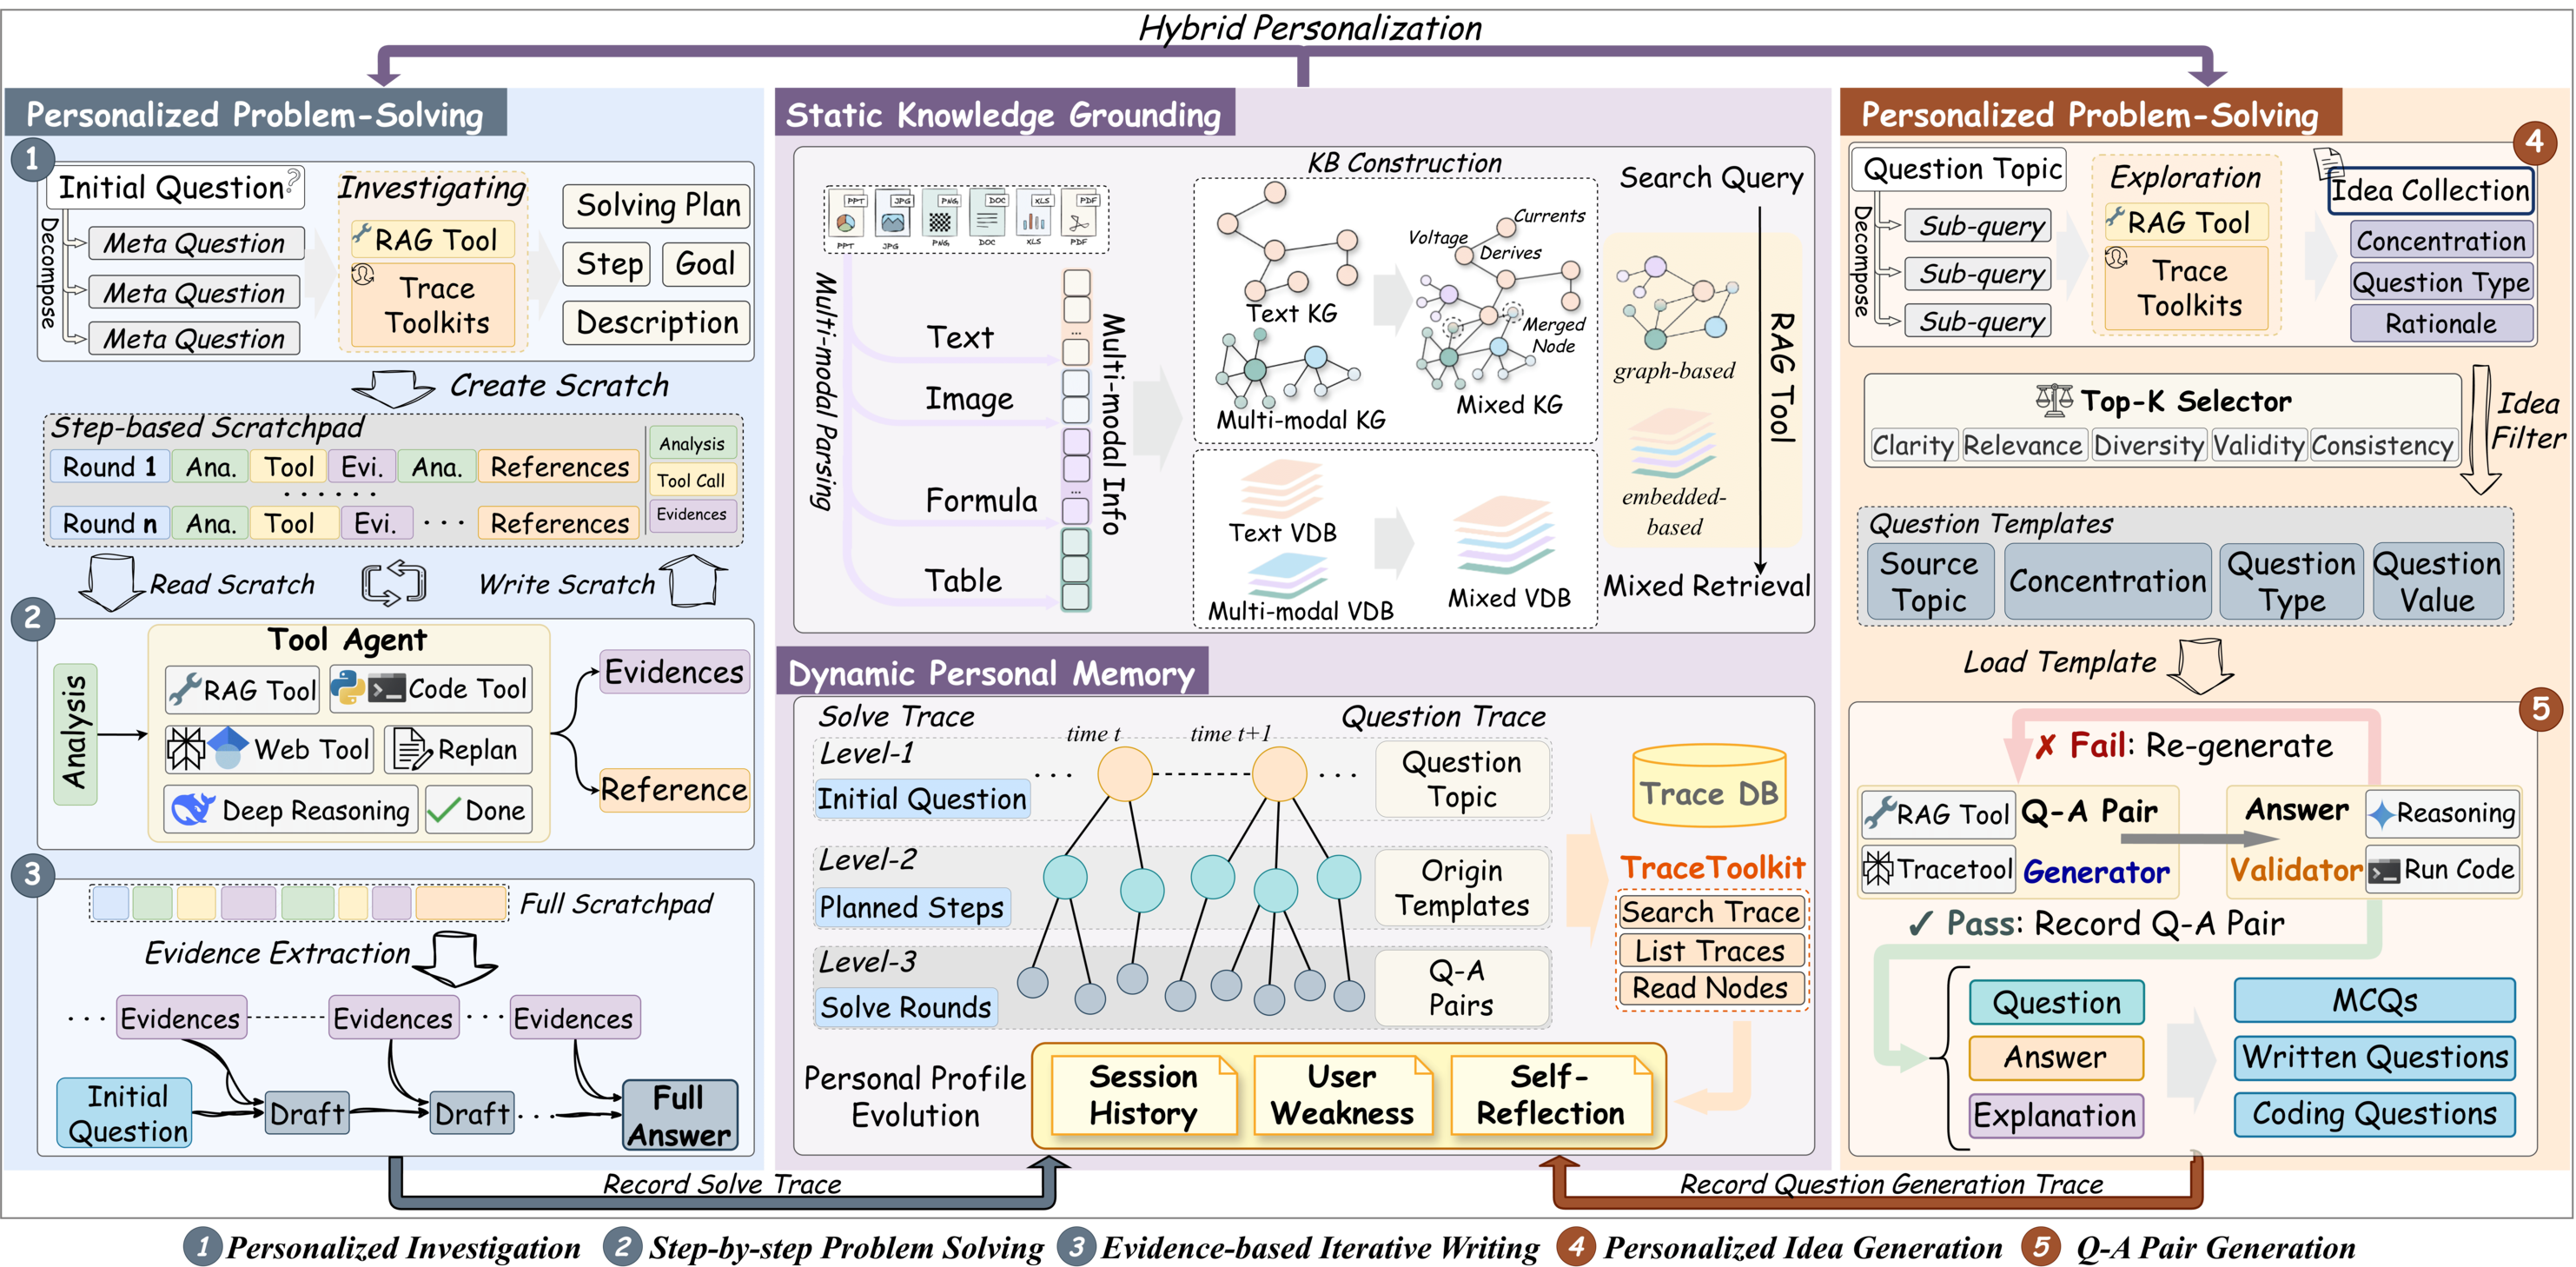
\includegraphics[width=\textwidth]{figures/full-pipe-0316.png}
    \caption{Overview of the personalization substrate and the foundational tutoring loop.
    A hybrid engine fuses static knowledge grounding (center) with dynamic personal memory (bottom).
    Problem solving (left, stages \ding{172}--\ding{174}) and question generation (right, stages \ding{175}--\ding{176}) form a closed cycle: both pipelines read from and write back to the shared learner profile.}
    \label{fig:overview}
\end{figure*}

An agentic tutoring system must do far more than answer isolated questions.
Learners solve problems, generate targeted practice, express understanding through writing, synthesize information from diverse sources, and absorb new concepts through structured engagement.
When these modalities are supported independently, the result is a disconnected toolkit: the writing agent forgets what the problem solver just diagnosed, and the question generator ignores what the learner struggled with yesterday.
Unifying all capabilities under a single, continuously evolving understanding of the individual learner is the organizing principle of this section.

\S\ref{sec:personalization} describes the personalization substrate.
\S\ref{sec:loop} presents the foundational tutoring loop coupling problem solving with question generation.
\S\ref{sec:cognitive_ext} extends this loop along three complementary dimensions of knowledge work.

% ===========================================================================
\subsection{The Personalization Substrate}
\label{sec:personalization}
% ===========================================================================

Effective tutoring demands two complementary forms of context: \emph{domain expertise} (what the course teaches) and \emph{learner awareness} (how the individual student has engaged with that material).
Domain knowledge tells the system what is important; learner awareness tells it what is important \emph{for this student, right now}.
The personalization engine supplies both through a static knowledge-grounding module and a dynamic personal memory, whose outputs are fused before every agent step.

\subsubsection{Static Knowledge Grounding}
\label{sec:rag}

Course materials are decomposed into atomic content units and indexed through two complementary structures~\citep{wang2024mineruopensourcesolutionprecise}.
A \emph{knowledge graph} $\mathcal{G}$ captures structural and conceptual relations among definitions, theorems, and examples, while dense encoders project all units into an \emph{embedding index} $\mathcal{B}$~\citep{guo2025raganythingallinoneragframework}.
The rationale for dual indexing is that educational queries span a continuum from structurally precise questions such as ``What are the prerequisites of Stokes' theorem?'' to semantically diffuse ones such as ``I'm confused about the relationship between circulation and flux.''
Graph traversal over $\mathcal{G}$ excels at the former, while dense search over $\mathcal{B}$ handles the latter.
The two candidate sets are fused via reciprocal rank fusion~\citep{cormack2009reciprocal}, deduplicated, and truncated to a context budget, yielding the domain grounding $\mathcal{C}_{\text{rag}}$.

\subsubsection{Dynamic Personal Memory: The Trace Forest}
\label{sec:memory}

Whereas static grounding captures \emph{what is taught}, dynamic memory captures \emph{how the individual has learned}.
The central representational challenge is how to remember months of tutoring interactions in a form that is simultaneously compact enough to fit in a context window and rich enough to inform future pedagogy.

We address this with the \emph{Trace Forest}~$\mathcal{F}$, a hierarchical, multi-resolution data structure in which each tree records one complete tutoring interaction as a semantically searchable artifact.
Nodes are organized into three levels of granularity.
\emph{Level~1} stores session-level metadata and a global summary, capturing the overall topic, outcome, and duration of the interaction.
\emph{Level~2} captures intermediate planning units produced during task decomposition, each recording a sub-goal, its status, and a condensed rationale.
\emph{Level~3} preserves fine-grained execution records, including tool outputs, retrieved evidence, and validation outcomes.
Every node carries a dense embedding computed from its textual content, enabling similarity-based retrieval across the entire forest~\citep{packer2023memgpt,qin2025himem,yang2025gmemory}.

A new trace tree is created at the end of each tutoring session.
The three-level structure is populated incrementally as the session progresses: the planner creates Level~2 nodes when it decomposes a problem, the executor appends Level~3 nodes as it processes each sub-goal, and a post-session summarizer generates the Level~1 root from the completed tree.

The multi-resolution design reflects a deliberate trade-off between flat conversation logs (easy to store but expensive to search) and fixed-size summaries (compact but detail-lossy).
The three-level hierarchy allows the system to operate at the right resolution for each task: session summaries for long-range trends, planning-level nodes for conceptual trajectories, and execution-level nodes for recalling exactly \emph{how} a student arrived at a particular misunderstanding.

Rather than treating $\mathcal{F}$ as a passive archive, we expose it through a programmatic \emph{TraceToolkit} with three operations:
\textsc{SearchTrace} performs semantic retrieval across all trees and levels, ranking nodes by embedding similarity to the current query and returning results with their ancestry paths so that fine-grained nodes can be interpreted in the context of their parent session.
\textsc{ListTraces} supports filtered enumeration by time range, topic, or outcome, enabling agents to quickly survey recent activity or locate sessions on a particular subject.
\textsc{ReadNodes} provides full-content access to one or more nodes together with ancestry-path reconstruction, allowing an agent to drill down from a session summary to the exact execution record that produced a specific misconception diagnosis.
This toolkit is available to every agent in the system, making past interactions a first-class resource that can be consulted as readily as the knowledge base itself.

\subsubsection{Profile Construction and Injection}
\label{sec:injection}

Three specialized memory agents process each new trace in parallel, each maintaining one dimension of the learner profile $\mathcal{D} = (\mathcal{D}_s, \mathcal{D}_w, \mathcal{D}_r)$:
\begin{itemize}[nosep,leftmargin=*]
\item \textbf{Session History} $\mathcal{D}_s$: a running account of topics covered and performance trends.
The session-history agent extracts the subject, difficulty level, and outcome of each session and appends a dated entry to $\mathcal{D}_s$, enabling downstream agents to identify long-range patterns such as topics that recur frequently or performance trajectories that plateau.
\item \textbf{Weakness Diagnosis} $\mathcal{D}_w$: a prioritized inventory of knowledge gaps, each labeled as \emph{active} or \emph{resolved}.
The weakness agent examines execution-level nodes for evidence of confusion, incorrect reasoning steps, or repeated errors, and either creates a new gap entry or updates an existing one.
A gap is labeled \emph{resolved} when the student demonstrates correct application across at least two subsequent sessions; it reverts to \emph{active} if later evidence shows the misconception has resurfaced.
\item \textbf{Self-Reflection} $\mathcal{D}_r$: the system's pedagogical self-critique, consisting of actionable notes on what explanatory strategies worked well and what to improve.
The reflection agent compares the tutor's intended approach with the student's actual responses, noting instances where scaffolding was too sparse or too dense, where analogies succeeded or confused, and where the pacing mismatched the learner's readiness.
\end{itemize}

The three-dimensional decomposition is motivated by a pedagogical observation: effective tutoring requires knowing not only \emph{what} the student has done ($\mathcal{D}_s$) and \emph{where they struggle} ($\mathcal{D}_w$), but also \emph{how the tutor itself should adapt} ($\mathcal{D}_r$).
This self-reflective dimension is rare in existing systems; most treat the tutor as a fixed function of the student profile, ignoring the possibility that the tutoring strategy itself should evolve.

Before each agent step, a personalization context $\mathcal{C}_{\text{mem}}$ is assembled through two complementary channels.
First, \emph{active trace retrieval} uses the TraceToolkit to surface the most relevant nodes from $\mathcal{F}$, with retrieval budget allocated proportionally across the three levels.
Second, \emph{role-specific profile excerpting} routes different slices of $\mathcal{D}$ to different agents: the planner receives $\mathcal{D}_s$ and $\mathcal{D}_w$ to inform investigation strategy, the writer receives $\mathcal{D}_r$ to calibrate tone and depth, and the idea agent receives $\mathcal{D}_w$ to target practice at diagnosed gaps.
This selective injection prevents context saturation while ensuring that each agent receives precisely the personalization signal it needs.

% ===========================================================================
\subsection{Closing the Tutoring Loop}
\label{sec:loop}
% ===========================================================================

A personalization substrate is only as valuable as the feedback loop that keeps it current.
The foundational tutoring loop couples two complementary pipelines, problem solving and question generation, through the shared learner model.

\paragraph{Why two pipelines, and why coupled?}
A tutor that only answers questions never challenges the student's blind spots; a system that only generates practice is an exercise book, not a tutor.
Coupling the two makes the system pedagogically complete: weaknesses diagnosed during problem solving propagate to $\mathcal{D}_w$ and shape which questions are generated next, while the learner's performance on those questions refines $\mathcal{D}_s$ and $\mathcal{D}_r$, improving future explanations.

\paragraph{Personalized Problem Solving.}
The problem-solving pipeline separates concerns that compete for the same context window into three sequential agent stages.
\emph{Stage~\ding{172}, Personalized Investigation}, decomposes the student's question into meta-questions, gathers evidence from both $\mathcal{C}_{\text{rag}}$ and $\mathcal{C}_{\text{mem}}$, and synthesizes a solving plan tailored to the individual's gaps.
This ensures that personalization enters the pipeline at the earliest possible stage rather than being retrofitted during writing.
\emph{Stage~\ding{173}, Step-by-Step Solving}, executes each sub-goal through a think--act--observe loop~\citep{yao2023reactsynergizingreasoningacting} with self-notes and hierarchical compression to manage context growth, plus adaptive replanning when evidence reveals the current plan is inadequate.
\emph{Stage~\ding{174}, Evidence-Based Writing}, constructs the final answer through iterative draft--refine passes, using the learner profile $\mathcal{D}$ to calibrate depth and tone.
Beginners receive scaffolded derivations~\citep{wood1976role}, while proficient learners receive concise insights.
Every claim carries a traceable citation to retrieved evidence.

The rationale for this three-stage decomposition is that investigation, execution, and presentation serve fundamentally different cognitive functions and compete for the same limited context budget.
Prior approaches that fold all three into a single reasoning loop~\citep{yao2023reactsynergizingreasoningacting,wu-etal-2025-agentic} sacrifice either investigation depth or presentation quality as the problem grows complex.

\paragraph{Personalized Question Generation.}
Question generation is decomposed into two stages that separate \emph{what to ask} from \emph{how to ask and verify}.
\emph{Stage~\ding{175}, Idea Generation}, maps the conceptual landscape around a topic through the lens of the individual learner, producing candidate question ideas with personalized rationales grounded in diagnosed gaps from $\mathcal{D}_w$.
An evaluator-driven filtering-then-ranking pass prunes ill-formed or redundant candidates.
\emph{Stage~\ding{176}, Critic-Guided Generation}, instantiates each idea into a question--answer--explanation triple, verified by a structurally separated validator that checks template alignment, factual correctness, and, for computational questions, sandboxed code execution.
Because the validator shares no reasoning chain with the generator, it must independently verify correctness, reducing self-confirming errors~\citep{spiliopoulou2025playfavorites}.

\paragraph{The Closed-Loop Dynamic.}
\label{sec:cycle}
After each interaction, the system appends a new trace tree to $\mathcal{F}$ and the three memory agents update $\mathcal{D}$ in parallel.
The key property is \emph{bidirectional task coupling}: the solving pipeline feeds the generation pipeline through $\mathcal{D}_w$, and the generation pipeline feeds back into the solving pipeline through $\mathcal{D}_s$ and $\mathcal{D}_r$.
Because every agent can query the trace forest at any time, this feedback extends beyond profile-level summaries to fine-grained precedents from any prior interaction, enabling increasingly nuanced personalization as the interaction history grows.
The complete closed-loop algorithm is provided in Appendix~\ref{app:algorithm}.

% ===========================================================================
\subsection{Beyond Q\&A: Cognitive Extension across Knowledge Modalities}
\label{sec:cognitive_ext}
% ===========================================================================

\begin{figure}[t]
    \centering
    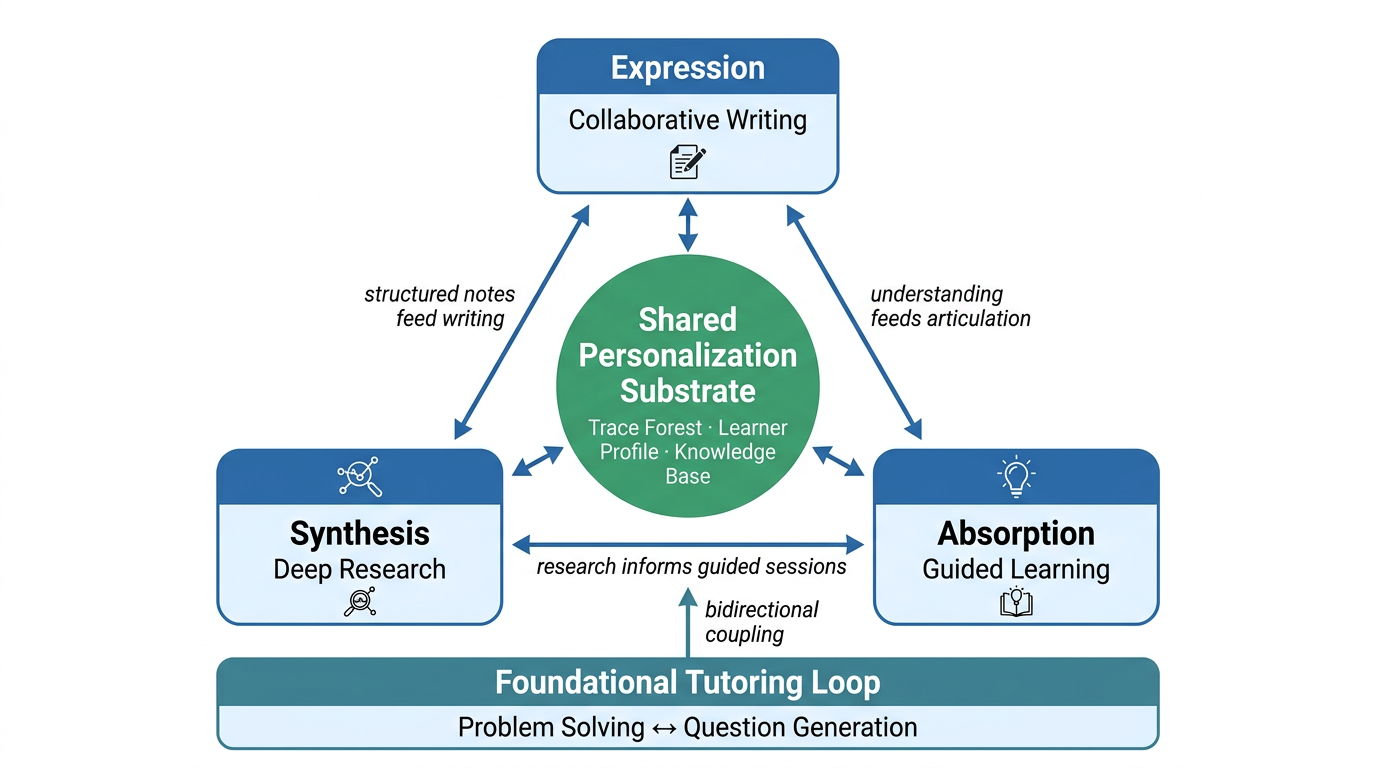
\includegraphics[width=\columnwidth]{figures/cognitive-extension.png}
    \caption{Three cognitive extensions, \emph{expression}, \emph{synthesis}, and \emph{absorption}, extend the tutoring loop into a broader support cycle. All three share the same personalization substrate, so progress in any modality informs the others.}
    \label{fig:extension}
\end{figure}

The tutoring loop of~\S\ref{sec:loop} covers the most familiar form of learning, but real learning extends beyond asking and answering.
Learners also \emph{express} understanding through writing, \emph{synthesize} information from diverse sources, and \emph{absorb} new concepts through active engagement (Figure~\ref{fig:extension}).
The key design question is how to support these modalities without fragmenting the learner's experience; our answer is to run every extension on the same personalization substrate.

\paragraph{Knowledge Expression: Collaborative Writing.}
An \texttt{EditAgent} operates in a tool-augmented loop: given a document context and an editing instruction, it retrieves relevant passages via RAG, gathers supplementary information through web search when needed, and produces structured edits with inline citations.
Access to $\mathcal{C}_{\text{mem}}$ lets it calibrate assistance to the individual, providing scaffolded guidance for beginners and concise refinements for advanced writers.
Every writing session generates a trace that captures the topics chosen and the structural weaknesses encountered, enriching the learner profile for all downstream capabilities.

\paragraph{Knowledge Synthesis: Multi-Agent Deep Research.}
When learners move from coursework to independent study, they need to construct knowledge by integrating information from many sources, a task that demands multi-step agentic orchestration rather than single-turn generation.
The deep research capability addresses this through a four-stage multi-agent pipeline.
First, the user's query is rephrased and decomposed into topics.
Multiple \texttt{ResearchAgent} instances then operate concurrently, each drawing on the full tool suite including knowledge-base retrieval, web search, academic paper search, and sandboxed code execution.
A manager agent dynamically injects emergent sub-topics discovered during investigation, allowing the research to follow threads that were not anticipated at decomposition time.
Finally, the pipeline generates output in one of four modes, \emph{comprehensive}, \emph{focused}, \emph{comparative}, or \emph{exploratory}, reflecting distinct cognitive needs. A student surveying a new field needs landscape notes rather than a lengthy report, while a student choosing between two frameworks needs a comparative analysis rather than an exhaustive survey.

\paragraph{Knowledge Absorption: Interactive Guided Learning.}
Problem solving and research are student-initiated; guided learning inverts this dynamic by having the system lead the learner through structured, active engagement, a mode shown to dramatically outperform passive reading~\citep{freeman2014active}.
The capability is realized through a three-agent pipeline.
A \texttt{DesignAgent} creates a structured learning plan calibrated to diagnosed weak points from $\mathcal{D}_w$, identifying key concepts, prerequisite relationships, common misconceptions, and an appropriate difficulty progression.
An \texttt{InteractiveAgent} then leads the student through the plan via Socratic multi-turn dialogue, introducing concepts progressively, posing probing questions, and providing scaffolded hints rather than direct answers.
After the session, a \texttt{SummaryAgent} generates a synthesis of knowledge points covered and areas for follow-up, enriching the trace forest for all future interactions.

\paragraph{Cross-Modality Coherence.}
Because all three modalities share the same trace forest and learner profile, they form a mutually reinforcing cycle without explicit cross-modality wiring.
Weaknesses surfaced during problem solving inform guided sessions; insights from guided learning improve research strategies; and structured notes from deep research feed back into writing assistance.
